\chapter{Развёртка структур данных}
\label{ch:10}

Английское слово \textit{bootstrapping}\translationnote{%
  Я перевожу это слово как <<развёртка>>. Каламбур при этом, к
  сожалению, теряется.%
} 
означает <<процесс приподнимания самого себя за шнурки
ботинок>>. Этот, казалось бы, бессмысленный образ описывает
распространённую в информатике ситуацию, когда, чтобы решить задачу,
нам нужно иметь готовое решение той же самой задачи (в какой-то её
более простой разновидности).

Рассмотрим, например, процесс загрузки операционной системы в
компьютер с диска или магнитной ленты. Без операционной системы
компьютер не может даже обратиться к диску или ленте! Решением будет
\term{начальный загрузчик}{bootstrap loader}~--- крошечная, неполная
операционная система, чьей единственной целью является чтение немного
более крупной и мощной операционной системы и передача ей
управления. Та, в свою очередь, считывает настоящую операционную
систему и передает управление уже ей. Можно рассматривать эту картину
как пример развёртки полного решения на основе неполного.

Ещё одним примером может служить развёртка компилятора. Часто бывает,
что компилятор с нового языка пишется на самом этом языке. Но как
тогда скомпилировать этот компилятор? Одно из возможных решений~--- написать простой,
неэффективный интерпретатор нового языка на каком-либо старом
существующем языке. С помощью этого интерпретатора компилятор применяется
к своему собственному коду, и получается эффективный компилятор в
виде скомпилированного кода. Можно рассматривать это как пример
развёртки эффективного решения на основе неэффективного.

Адам Бухсбаум в своей диссертации \cite{Buchsbaum1993} описывает две
методики разработки алгоритмов, которые он вместе называет
\term{развёртка структур данных}{data-structural
  bootstrapping}. Первая методика, \term{структурная
  декомпозиция}{structural decomposition}, предназначена для развёртки
неполных структур данных, чтобы получить полные. Вторая методика,
\term{структурная абстракция}{structural abstraction}, используется
для развёртки неэффективных структур данных в эффективные. В этой
главе мы заново рассматриваем обе этих методики и добавляем к ним
третью, позволяющую развёртывать структуры данных с простейшими
элементами и получать структуры с составными элементами.

\section{Структурная декомпозиция}
\label{sc:10.1}

\term{Структурная декомпозиция}{structural decomposition}~--- это
метод для получения полных структур данных на основе неполных.  Как
правило, берется реализация, способная работать только с объектами
ограниченного размера (может быть, даже только нулевого размера), и
расширяется так, чтобы работать с объектами неограниченного размера.

Рассмотрим типичные рекурсивные типы данных, например, списки и
двоичные листовые деревья.
\begin{lstlisting}
  datatype $\alpha$ List = Nil | Cons of $\alpha$ $\times$ $\alpha$ List
  datatype $\alpha$ Tree = Leaf of $\alpha$ | Node of $\alpha$ Tree $\times$ $\alpha$ Tree
\end{lstlisting}
При желании их можно рассматривать как примеры структурной
декомпозиции. И то, и другое определение состоит из простой реализации
для объектов ограниченного размера (ноль для списков и один для
деревьев) плюс правило для рекурсивной декомпозиции более крупных
объектов в более мелкие, пока, в конце концов, все объекты не окажутся
достаточно маленькими, чтобы с ними справилось базовое правило.

Однако оба этих определения просты ещё и в том, что рекурсивная
компонента каждого определения совпадает с определяемым
типом. Например, рекурсивная компонента определения
\lstinline!$\alpha$ List! также является \lstinline!$\alpha$ List!. 
Такой тип называется \term{гомогенно рекурсивным}{uniformly
  recursive}.

Как правило, мы используем термин \emph{структурная декомпозиция} для
описания структур данных, которые являются
\term{гетерогенными}{non-uniform}. Рассмотрим, например, такое
определение последовательностей:
\begin{lstlisting}
  datatype $\alpha$ Seq = Nil' | Cons' of $\alpha$ $\times$ ($\alpha$ $\times$ $\alpha$) Seq
\end{lstlisting}
Здесь последовательность может быть либо пустой, либо состоять из
элемента и последовательности пар элементов. Рекурсивная компонента
\lstinline!($\alpha$ $\times$ $\alpha$) Seq! отличается от
\lstinline!$\alpha$ Seq!, так что этот тип гетерогенен.

Почему мы можем предпочитать гетерогенное определение гомогенному?
Часто гетерогенные типы за счёт своей более изощренной структуры поддерживают
более эффективные алгоритмы, чем их гомогенные аналоги. Сравним,
например, следующие функции определения размера для списков и
последовательностей:
\begin{lstlisting}
  fun sizeL Nil = 0
    | sizeL (Cons (x, xs)) = 1 + sizeL xs

  fun sizeS Nil' = 0
    | sizeS (Cons' (x, ps)) = 1 + 2 * sizeS ps
\end{lstlisting}
Функция для списков требует время $O(n)$, в то время как функция для
последовательностей требует $O(\log n)$.

\subsection{Гетерогенная рекурсия и Стандартный ML}
\label{sc:10.1.1}

К сожалению, как правило, мы не можем выразить структурную
декомпозицию напрямую на Стандартном ML. Несмотря на то, что
Стандартный ML позволяет определять гетерогенные рекурсивные типы
данных, система типов запрещает большинство интересных функций на
основе этих типов. Рассмотрим, например, функцию \lstinline!sizeS! для
последовательностей. Эта функция будет отвергнута компилятором
Стандартного ML, поскольку система типов требует, чтобы все
рекурсивные вызовы в теле рекурсивной функции имели тот же тип, что и
объемлющая функция (т.~е., рекурсивные определения функций должны быть
гомогенны). Функция \lstinline!sizeS! нарушает это ограничение,
поскольку внешнее вхождение \lstinline!sizeS! имеет тип 
\lstinline!$\alpha$ Seq $\to$ int!, а внутреннее~--- тип 
\lstinline!($\alpha$ $\times$ $\alpha$) Seq $\to$ int!.

Всегда можно преобразовать гетерогенный тип в гомогенный, введя новый
тип данных, который сливает различные употребления в один
тип. Например, сливая элементы и пары элементов, можно переписать тип
\lstinline!Seq! в виде
\begin{lstlisting}
  datatype $\alpha$ EP = Elem of $\alpha$ | Pair of $\alpha$ EP $\times$ $\alpha$ EP
  datatype $\alpha$ Seq = Nil' | Cons' of $\alpha$ EP $\times$ $\alpha$ Seq
\end{lstlisting}
В таком случае \lstinline!sizeS! оказывается совершенно законной в том
виде, как она исходно была записана; как внешний вызов
\lstinline!sizeS!, так и внутренний имеют тип 
\lstinline!$\alpha$ Seq $\to$ int!.

Поскольку гетерогенный тип всегда можно преобразовать в гомогенный,
термин <<структурная декомпозиция>> относится скорее к способу нашего
рассуждения о типе данных, чем к его реализации. Рассмотрим, например,
модифицированное определение типа \lstinline!Seq!, приведенное
выше. Тип \lstinline!$\alpha$ Seq! изоморфен двоичным листовым
деревьям, так что модифицированная версия \lstinline!$\alpha$ Seq!
эквивалентна \lstinline!$\alpha$ Tree list!. Однако, как правило, мы
думаем о списке деревьев иначе, чем о последовательности пар~---
некоторые алгоритмы кажутся проще или естественнее в одном
представлении, другие в другом. В следующем разделе мы увидим
несколько примеров.

Есть также несколько практических соображений, заставляющих нас
предпочитать гетерогенное определение \lstinline!$\alpha$ Seq!
гомогенному. Во-первых, оно короче; имеется один тип, а не два, и
незачем всюду вручную расставлять конструкторы \lstinline!Elem! и
\lstinline!Pair!. Во-вторых, в некоторых реализациях языка
гетерогенное определение может быть эффективнее: нет необходимости
проводить сопоставление с конструкторами \lstinline!Elem! и
\lstinline!Pair!, и незачем во время выполнения строить в памяти
представления этих конструкторов. В-третьих, и это самое важное
соображение, гетерогенное определение позволяет системе типов
отлавливать намного больше программистских ошибок. Тип в гетерогенном
определении обеспечивает инвариант, что внешний конструктор
\lstinline!Cons'! содержит один элемент, второй пару элементов, третий
пару пар, и так далее. Тип гомогенного определения не гарантирует ни
баланса в парах, ни увеличения глубины пар по одному на уровень. Эти
ограничения должны обеспечиваться программистом как инварианты
системы. Но если программист ненамеренно нарушит эти инварианты~---
например, использовав элемент там, где ожидается пара,~--- система
типов не поможет ему поймать эту ошибку.

Исходя из этих соображений, мы часто представляем код так, как если бы
Стандартный ML  поддерживал гетерогенные рекурсивные определения
функций, известные также как \term{полиморфная рекурсия}{polymorphic
  recursion} \cite{Mycroft1984}. Наш код будет невозможно напрямую
выполнить, но он будет более читаемым. Его всегда можно преобразовать
обратно в законный Стандартный ML, используя приёмы, описанные пару
абзацев назад.

\subsection{Снова двоичные списки с произвольным доступом}
\label{sc:10.1.2}

При всех своих достоинствах, обсуждаемый нами тип 
\lstinline!$\alpha$ Seq! бесполезен для представления последовательностей. Проблема в том,
что он может представлять только последовательности длиной $2^k -
1$. Если использовать терминологию числовых представлений, конструктор
\lstinline!Cons'! позволяет нам записывать биты-единицы, но не
биты-нули. Это легко исправить, добавив в тип ещё один
конструктор. Кроме того, мы переименовываем конструктор
\lstinline!Cons'!, чтобы подчеркнуть аналогию с двоичными числами.
\begin{lstlisting}
  datatype $\alpha$ Seq = Nil | Zero of ($\alpha$ $\times$ $\alpha$) Seq | One of $\alpha$ $\times$ ($\alpha$ $\times$ $\alpha$) Seq
\end{lstlisting}
Теперь последовательность 0\ldots 10 можно представить как
\begin{lstlisting}
  One (0, One ((1,2), Zero (One ((((3,4),(5,6)),((7,8),(9,10))), Nil))))
\end{lstlisting}
Размер этой последовательности 11, что в двоичном виде записывается
как \texttt{1101}.

Пары в этом типе всегда сбалансированы. В сущности, можно думать о
парах элементов или о парах пар элементов и т.~д. как о полных
двоичных листовых деревьях. Таким образом, наш тип, по существу,
эквивалентен типу двоичных списков с произвольным доступом из
Раздела~\ref{sc:9.2.1}, но только с явно представленными инвариантами.

Давайте заново реализуем функции двоичных списков с произвольным
доступом, на этот раз рассуждая в терминах элементов и
последовательностей пар, а не в терминах списков полных двоичных
листовых деревьев. Функции по-прежнему будут работать за время $O(\log
n)$, однако, как мы сейчас увидим, новый способ мышления, как правило,
даёт нам более короткие и понятные алгоритмы.

Начнём с функции \lstinline!cons!. Первые два варианта не представляют
трудности:
\begin{lstlisting}
  fun cons (x, Nil) = One (x, Nil)
    | cons (x, Zero ps) = One (x, ps)
\end{lstlisting}
Чтобы добавить элемент к последовательности, имеющей вид 
\lstinline!One (y, ps)!, мы строим пару из нового и существующего
элементов, и добавляем её в последовательность пар.
\begin{lstlisting}
  fun cons (x, One (y, ps)) = Zero (cons ((x, y), ps))
\end{lstlisting}
Здесь требуется полиморфная рекурсия: внешний \lstinline!cons! имеет
тип
$$
\lstinline!$\alpha$ $\times$ $\alpha$ Seq $\to$ $\alpha$ Seq!
$$
а внутренний \lstinline!cons! имеет тип
$$
\lstinline!($\alpha$ $\times$ $\alpha$) $\times$ ($\alpha$ $\times$ $\alpha$) Seq $\to$ ($\alpha$ $\times$ $\alpha$) Seq!
$$

Мы реализуем функции \lstinline!head! и \lstinline!tail! через
вспомогательную функцию \lstinline!uncons!, разбивающую
последовательность на первый элемент и последовательность остальных
элементов.
\begin{lstlisting}
  fun head xs = let val (x, _) = uncons xs in x end
  fun tail xs = let val (_, xs') = uncons xs' in xs' end
\end{lstlisting}
Функция \lstinline!uncons! получается путём прочтения
всех строчек \lstinline!cons! справа налево.
\begin{lstlisting}
  fun uncons (One (x, Nil)) = (x, Nil)
    | uncons (One (x, ps)) = (x, Zero ps)
    | uncons (Zero ps) = let val ((x, y), ps') = uncons ps
                         in (x, One (y, ps')) end
\end{lstlisting}

Рассмотрим теперь функцию \lstinline!lookup!. Получив
последовательность \lstinline!One (x, ps)!, мы либо возвращаем
\lstinline!x!, либо переадресуем запрос к \lstinline!Zero ps!.
\begin{lstlisting}
  fun lookup (0, One (x, ps)) = x
    | lookup (i, One (x, ps)) = lookup (i-1, Zero ps)
\end{lstlisting}
Чтобы найти элемент по индексу $i$ в списке пар, мы находим пару по
индексу $\lfloor i/2 \rfloor$, а затем извлекаем нужный элемент из
этой пары.
\begin{lstlisting}
  fun lookup (i, Zero ps) = let val (x, y) = lookup (i div 2, ps)
                            in if i mod 2 = 0 then x else y end
\end{lstlisting}

Наконец, рассмотрим функцию \lstinline!update!. Варианты для
конструктора \lstinline!One! выглядят просто:
\begin{lstlisting}
  fun update (0, e, One (x, ps)) = One (e, ps)
    | update (i, e, One (x, ps)) = cons (x, update (i-1, e, Zero ps))
\end{lstlisting}
Однако пытаясь обновить элемент в последовательности пар, мы
сталкиваемся с небольшой проблемой. Нам нужно обновить пару по индексу
$\lfloor i/2 \rfloor$, но, чтобы создать новую пару, требуется второй
элемент старой пары. Поэтому прежде, чем рекурсивно вызвать
\lstinline!update!, нам приходится звать \lstinline!lookup!.
\begin{lstlisting}
  fun update (i, e, Zero ps) = 
  let val (x, y) = lookup (i div 2, ps)
      val p = if i mod 2 = 0 then (e, y) else (x, e)
  in Zero (update (i-1, p, ps)) end
\end{lstlisting}

\begin{exercise}\label{ex:10.1}
  Докажите, что эта версия \lstinline!update! работает за время
  $O(\log^2 n)$.
\end{exercise}

Чтобы восстановить ограничение $O(\log n)$ для функции
\lstinline!update!, надо избавиться от вызова
\lstinline!lookup!. Но как тогда мы получим второй элемент, который
нам нужен для построения новой пары? Если мы не можем привести
Магомета к горе, придётся вести гору к Магомету. А именно, вместо
того, чтобы получать старую пару и локально конструировать новую, мы
строим функцию для построения новой пары из старой, когда эта старая
пара будет найдена. Используем вспомогательную функцию
\lstinline!fupdate!, принимающую в качестве аргумента функцию, которую
требуется применить к $i$-му элементу последовательности. В этом
случае \lstinline!update! выглядит просто как
\begin{lstlisting}
  fun update (i, y, xs) = fupdate(fn x $\Rightarrow$ y, i, xs)
\end{lstlisting}
Ключевым шагом в \lstinline!fupdate! будет преобразование функции
\lstinline!f! на элементах в функцию \lstinline!f'!, принимающую пару
элементов, и, в зависимости от чётности \lstinline!i!, применяющую
\lstinline!f! либо к первому, либо ко второму элементу пары.
\begin{lstlisting}
  fun f' (x, y) = if i mod 2 = 0 then (f x, y) else (x, f y)
\end{lstlisting}
Имея это определение, уже нетрудно написать оставшуюся часть
\lstinline!fupdate!.
\begin{lstlisting}
  fun fupdate (f, 0, One (x, ps)) = One (f x, ps)
    | fupdate (f, i, One (x, ps)) = cons (x, fupdate (f, i-1, Zero ps))
    | fupdate (f, i, Zero ps) =
        let fun f' (x, y) = if i mod 2 = 0 then (f x, y) else (x, f y)
        in Zero (fupdate (f', i div 2, ps)) end
\end{lstlisting}
Полная реализация приведена на Рис.~\ref{fig:10.1}.

\begin{figure}
  \centering
  
  \caption{Альтернативная реализация двоичных списков с произвольным доступом.}
  \label{fig:10.1}
\end{figure}

При сравнении Рис.~\ref{fig:10.1} и Рис.~\ref{fig:9.6} мы видим, что
новая реализация намного короче и что все функции заметно проще; может
быть, за исключением \lstinline!update!. (А если мы не боимся функций
высших порядков, то даже \lstinline!update! выглядит проще.) Все эти
преимущества получены потому, что мы представили структуру данных
в виде гетерогенного типа, прямо отражающего искомые инварианты.

\begin{exercise}\label{ex:10.2}
  Модифицируйте \lstinline!AltBinaryRandomAccessList!, чтобы
  \lstinline!cons!, \lstinline!head! и \lstinline!tail! работали за
  амортизированное время $O(1)$, используя тип
  \begin{lstlisting}
    datatype $\alpha$ RList = 
           Nil
         | One of $\alpha$ $\times$ ($\alpha$ $\times$ $\alpha$) RList susp
         | Two of $\alpha$ $\times$ $\alpha$ $\times$ ($\alpha$ $\times$ $\alpha$) RList susp
         | Three of $\alpha$ $\times$ $\alpha$ $\times$ $\alpha$ $\times$ ($\alpha$ $\times$ $\alpha$) RList susp
  \end{lstlisting}
\end{exercise}

\subsection{Развёрнутые очереди}
\label{sc:10.1.3}

Рассмотрим использование $\concat$ в очередях по методу банкира из
Раздела~\ref{sc:6.3.2}. Во время проворота очереди головной поток
\lstinline!f! заменяется потоком \lstinline!f $\concat$ reverse r!. 
После последовательности проворотов головной поток имеет вид
$$
\lstinline!((f $\concat$ reverse r$_1$) $\concat$ reverse r$_2$) $\concat$ $\cdots$ $\concat$ reverse r$_k$!
$$
Хорошо известно, что \lstinline!append! в таких левоассоциативных
контекстах неэффективен, поскольку он многократно обрабатывает
элементы потоков, расположенных слева. Например, в этом случае
элементы \lstinline!f! будут обработаны $k$ раз (по разу на каждое
вхождение $\concat$), а элементы \lstinline!r$_i$! будут обработаны $k
-i + 1$ раз (один раз при выполнении \lstinline!reverse!, а затем по
разу на каждое $\concat$ справа). В общем случае левоассоциативная
конкатенация легко ведет к квадратичному поведению. К счастью, в нашем
случае общая стоимость всех конкатенаций по-прежнему линейна,
поскольку каждый \lstinline!r$_i$! по меньшей мере вдвое длиннее
предыдущего. Однако повторная обработка иногда на практике делает эти
очереди слишком медленными. Сейчас мы исправим этот
недостаток с помощью структурной декомпозиции.

Считая, что передний поток имеет вышеописанную структуру, мы разбиваем
его на две части: \lstinline!f! и коллекцию 
$m = \{\lstinline!reverse r$_1$!, \ldots, \lstinline!reverse r$_k$!\}$. 
Мы можем теперь представлять \lstinline!f! в виде списка, а каждый из
\lstinline!reverse r$_i$! как задержанный список. Кроме того,
хвостовой поток \lstinline!r! мы тоже заменяем на список. Эти
преобразования уничтожают подавляющее большинство задержек, и нам
удается избежать почти всех расходов, связанных с ленивым
вычислением. Но как нам представить коллекцию $m$? Как мы увидим,
доступ к этой коллекции происходит по правилу FIFO, так что, используя
структурную декомпозицию, мы можем её представить как очередь
задержанных списков.  Как и в любом рекурсивном типе, нам нужно
основание рекурсии, так что пустые очереди мы представляем через
особый конструктор.\footnote{%
  Немного более эффективным вариантом было бы представлять очереди,
  меньшие определенного фиксированного размера, как обыкновенные списки.%
}
Следовательно, наше новое представление будет
\begin{lstlisting}
  datatype $\alpha$ Queue =
       E | Q of int $\times$ $\alpha$ list $\times$ $\alpha$ list susp Queue $\times$ int $\times$ $\alpha$ list
\end{lstlisting}
Первое целое число, \lstinline!lenfm!, представляет собой совокупную
длину \lstinline!f! и всех задержанных списков в \lstinline!m! (т.~е.,
это величина, которая в старом представлении называлась просто
\lstinline!lenf!). Второе целое число, \lstinline!lenr!~--- это, как
обычно, просто длина \lstinline!r!. Обычный наш инвариант баланса
принимает вид $\lstinline!lenr! \le \lstinline!lenfm!$. Кроме того, мы
требуем, чтобы список \lstinline!f! был непустой. (В старом
представлении \lstinline!f! мог быть пуст, если пуста была вся
очередь, но теперь мы этот случай представляем отдельно.)

Как обычно, функции, работающие с очередью, написать нетрудно.
\begin{lstlisting}
  fun snoc (E, x) = Q (`, [x], E, 0, [])
    | snoc (Q (lenfm, f, m, lenr, r), x) = checkQ (lenfm, f, m, lenr+1, x::r)
  fun head (Q (lenfm, x :: f', m, lenr, r)) = x
  fun tail (Q (lenfm, x :: f', m, lenr, r)) = checkQ (lenfm-1, f', m, lenr, r)
\end{lstlisting}
Всё самое интересное содержится во вспомогательной функции
\lstinline!checkQ!. Если список \lstinline!r! слишком длинный, то
\lstinline!checkQ! создает задержку, которая должна развернуть
\lstinline!r! наоборот, а также оставляет задержку в \lstinline!m!.
После проверки длины \lstinline!r! функция \lstinline!checkQ! вызывает
вторую вспомогательную функцию \lstinline!checkF!, которая
гарантирует, что список \lstinline!f! непуст. Если пусты и
\lstinline!f!, и \lstinline!m!, то вся очередь пуста. В противном
случае, если пуст список \lstinline!f!, мы изымаем первую задержку из
\lstinline!m!, вынуждаем её и запоминаем получившийся список как
новую \lstinline!f!.
\begin{lstlisting}
  fun checkF (lenfm, [], E, lenr, r) = E
    | checkF (lenfm, [], m, lenr, r) =
        Q (lenfm, force (head m), tail m, lenr, r)
    | checkF q = Q q
  fun checkQ (q as (lenfm, f, m, lenr, r)) =
        if lenr <= lenfm then checkF q
        else checkF (lenfm+lenr, f, snoc (m, $\$$rev r),0, [])
\end{lstlisting}
Обратите внимание, что \lstinline!checkQ! и \lstinline!checkF!
вызывают \lstinline!snoc! и \lstinline!tail!, которые, в свою очередь,
зовут \lstinline!checkQ!. Следовательно, эти функции нужно определять
через взаимную рекурсию. Полная реализация приведена на
Рис.~\ref{fig:10.2}.

\begin{figure}
  \centering
  
  \caption{Развёрнутые очереди на основе структурной декомпозиции.}
  \label{fig:10.2}
\end{figure}

Эти очереди создают задержку, выполняющую обращение хвостового списка,
в тот же самый момент, что и очереди по методу банкира, а вынуждают её
на одну операцию раньше, чем очереди по методу банкира. Значит,
поскольку операция обращения добавляет только $O(1)$ амортизированного
времени к каждой операции в очередях по методу банкира, в наших
развёрнутых очередях она тоже добавляет только $O(1)$
амортизированного времени. Однако время выполнения \lstinline!snoc! и
\lstinline!tail! больше не является константой! Обратите внимание, что
\lstinline!snoc! вызывает \lstinline!checkQ!, а эта функция, в свою
очередь, может позвать \lstinline!snoc! для \lstinline!m!. Таким
образом, может возникнуть каскад вызовов \lstinline!snoc!, по одному
на каждом уровне очереди. Но последовательные списки в
\lstinline!m! по крайней мере удваиваются в размере, так что длина
\lstinline!m! равна $O(\log n)$. Поскольку длина срединной очереди
уменьшается по крайней мере на логарифмический множитель на каждом
уровне, глубина всей очереди не больше $O(\log^* n)$. \lstinline!snoc! на
каждом уровне производит $O(1)$ амортизированной работы, так что всего
\lstinline!snoc! требует $O(\log^* n)$ амортизированного времени.

Подобным образом, вызов \lstinline!tail! может привести к вызовам
как \lstinline!snoc! (из \lstinline!checkQ!), так и \lstinline!tail!
(из \lstinline!checkF!).  Заметим, что когда такое бывает,
\lstinline!tail! применяется к результату \lstinline!snoc!. Итак,
\lstinline!snoc! может рекурсивно себя вызвать, а \lstinline!tail!
может рекурсивно вызвать и \lstinline!snoc!, и
\lstinline!tail!. Однако из Упражнения~\ref{ex:10.3} мы знаем, что
никогда \lstinline!snoc! и \lstinline!tail! не вызывают
\lstinline!snoc! рекурсивно подряд. Следовательно, и \lstinline!snoc!,
и \lstinline!tail! зовутся максимум по разу на уровень.  Поскольку на
каждом уровне и \lstinline!snoc!, и \lstinline!tail! выполняют $O(1)$
амортизированной работы, общая амортизированная стоимость
\lstinline!tail! равна $O(\log^* n)$.

\begin{remark}
  На практике $O(\log^* n)$ является константой. Чтобы глубина
  достигла хотя бы пяти, очередь должна содержать не менее $2^{65536}$
  элементов. Более того, если представлять очереди до размера четыре
  просто в виде списков, то очереди с числом элементов примерно до четырёх
  миллиардов будут содержать не более трёх уровней.
\end{remark}

\begin{hint}
  На практике варианты этих очередей опережают все другие известные
  реализации в приложениях, где устойчивость используется умеренно,
  но требуется хорошее поведение даже в патологических случаях.
\end{hint}

\begin{exercise}\label{ex:10.3}
  Рассмотрим выражение \lstinline!tail (snoc (q, x))!. Покажите, что
  никогда не будет так, чтобы оба вызова, \lstinline!snoc! и
  \lstinline!tail!, рекурсивно обратились к \lstinline!snoc!.
\end{exercise}

\begin{exercise}\label{ex:10.4}
  Реализуйте эти очереди без использования полиморфной рекурсии, при
  помощи типов
  \begin{lstlisting}
    datatype $\alpha$ EL = Elem of $\alpha$ | List of $\alpha$ EL list susp
    datatype $\alpha$ Queue = E | Q of int $\times$ $\alpha$ EL list $\times$ $\alpha$ Queue $\times$ int $\times$ $\alpha$ EL list
  \end{lstlisting}
\end{exercise}

\begin{exercise}\label{ex:10.5}
  Ещё один способ избежать полиморфной рекурсии~--- представлять
  середину при помощи какой-либо другой реализации очередей. Тогда тип
  развёрнутых очередей будет
  \begin{lstlisting}
    datatype $\alpha$ Queue =
      E | Q of int $\times$ $\alpha$ list $\times$ $\alpha$ list susp PrimQ.Queue $\times$ int $\times$ $\alpha$ list
  \end{lstlisting}
  где \lstinline!PrimQ!~--- другая реализация очередей.
  \begin{enumerate}
  \item Реализуйте этот вариант развёрнутых очередей как функтор вида
    \begin{lstlisting}
      functor BootstrappedQueue (PrimQ: Queue): Queue = $\ldots$
    \end{lstlisting}
  \item Докажите, что если в качестве параметра \lstinline!PrimQ!
    выступает какая-либо реализация очередей реального времени, то все
    операции на развёрнутых очередях выполняются за амортизированное
    время $O(1)$.
  \end{enumerate}
\end{exercise}

\section{Структурная абстракция}
\label{sc:10.2}

Второй разновидностью развёртки структур данных является
\term{структурная абстракция}{structural abstraction}. Как правило,
она используется, чтобы расширить реализацию каких-либо коллекций,
скажем, списков или куч, эффективной функцией слияния для сочетания
двух коллекций. Во многих реализациях нетрудно построить эффективную
функцию \lstinline!insert!, которая добавляет в коллекцию один новый
элемент, но намного сложнее построить эффективную функцию
слияния. Структурная абстракция создает коллекции, содержащие другие
коллекции в качестве элементов. В таком случае, две коллекции можно
слить, просто вставив одну в другую.

Идею структурной абстракции можно почти полностью описать на уровне
типов. Допустим, имеется тип коллекций \lstinline!$\alpha$ C! с
элементами типа \lstinline!$\alpha$!, и этот тип поддерживает
эффективную функцию \lstinline!insert! с сигнатурой
\begin{lstlisting}
  val insert : $\alpha$ $\times$ $\alpha$ C $\to$ $\alpha$ C
\end{lstlisting}
Назовём \lstinline!$\alpha$ C!
\term{элементарным типом}{primitive type}.
На основе этого типа мы
хотим создать новый тип данных
\lstinline!$\alpha$ B!, называемый \term{развёрнутым
  типом}{bootstrapped type}, чтобы \lstinline!$\alpha$ B!
эффективно поддерживал и операцию \lstinline!insert!, и операцию
\lstinline!join!, с сигнатурами
\begin{lstlisting}
  val insert$_B$ : $\alpha$ $\times$ $\alpha$ B $\to$ $\alpha$ B
  val join$_B$ : $\alpha$ B $\times$ $\alpha$ B $\to$ $\alpha$ B
\end{lstlisting}
(С помощью нижнего индекса мы отличаем функции развёрнутого типа от
функций элементарного типа.) Кроме того, развёрнутый тип должен
поддерживать эффективную функцию \lstinline!unit! для создания новой
одноэлементной коллекции.
\begin{lstlisting}
  val unit$_B$ : $\alpha$ $\to$ $\alpha$ B
\end{lstlisting}
Тогда можно реализовать \lstinline!insert$_B$! просто как
\begin{lstlisting}
  fun insert$_B$ (x, b) = join$_B$ (unit$_B$ x, b)
\end{lstlisting}
Основная идея структурной абстракции состоит в том, чтобы представлять
развёрнутые коллекции как элементарные коллекции других развёрнутых
коллекций. Тогда можно реализовать \lstinline!join$_B$! через
\lstinline!insert! (а не \lstinline!insert$_B$!!) приблизительно как
\begin{lstlisting}
  fun join$_B$ (b$_1$, b$_2$) = insert (b$_1$, b$_2$)
\end{lstlisting}
Этот код вставляет \lstinline!b$_1$! в \lstinline!b$_2$! как
элемент. Можно также вставить \lstinline!b$_2$! как элемент в
\lstinline!b$_1$!; фокус в том, что мы свели \lstinline!join! к
простой вставке.

Разумеется, всё не так просто. На основе приведенного описания, мы
могли бы попытаться определить \lstinline!$\alpha$ B! как
\begin{lstlisting}
  datatype $\alpha$ B = B of ($\alpha$ B) C
\end{lstlisting}
Можно считать, что это определение задает гомоморфизм
$$
\lstinline!$\alpha$ B! \cong \lstinline!($\alpha$ B) C!
$$
Раскрыв этот гомоморфизм несколько раз, мы легко увидим ошибку в
определении.
$$
\lstinline!$\alpha$ B! \cong
\lstinline!($\alpha$ B) C! \cong
\lstinline!(($\alpha$ B) C) C! \cong
\cdots \cong
\lstinline!(($\cdots$ C) C) C!
$$
Тип \lstinline!$\alpha$! исчез, так что в нашей коллекции невозможно
хранить никакие элементы! Можно справиться с этой проблемой, если
сделать каждую развёрнутую коллекцию парой, состоящей из одного
элемента и элементарной коллекции.
\begin{lstlisting}
  datatype $\alpha$ B = B of $\alpha$ $\times$ ($\alpha$ B) C
\end{lstlisting}
Тогда, например, \lstinline!unit$_B$! можно определить как
\begin{lstlisting}
  fun unit$_B$ x = B (x, empty)
\end{lstlisting}
где \lstinline!empty!~--- пустая элементарная коллекция.

Однако теперь возникает ещё одна проблема. Если каждая развёрнутая
коллекция содержит по крайней мере один элемент, как мы представим
пустую развёрнутую коллекцию? Следовательно, мы снова исправляем тип.
\begin{lstlisting}
  datatype $\alpha$ B = E | B of $\alpha$ $\times$ ($\alpha$ B) C
\end{lstlisting}

\begin{remark}
  На самом деле, мы всегда устраиваем так, чтобы элементарная
  коллекция \lstinline!C! содержала только непустые развёрнутые
  коллекции. Эту ситуацию можно более точно описать с помощью типов
  \begin{lstlisting}
    datatype $\alpha$ B$^+$ = B$^+$ of $\alpha$ $\times$ ($\alpha$ B$^+$) C
    datatype $\alpha$ B = E | NE of B$^+$
  \end{lstlisting}
  К сожалению, определения такого вида ведут к более многословным
  программам, так что мы продолжаем использовать менее точное, но
  более короткое определение.
\end{remark}

Теперь можно уточнить шаблоны функций \lstinline!insert$_B$! и
\lstinline!join$_B$!:
\begin{lstlisting}
  fun insert$_B$ (x, E) = B (x, empty)
    | insert$_B$ (x, B (y, c)) = B (x, insert (unit$_B$ y, c))

  fun join$_B$ (b, E) = b
    | join$_B$ (E, b) = b
    | join$_B$ (B (x, c), b) = B (x, insert (b, c))
\end{lstlisting}
В этих шаблонах можно легко изменить различные детали. Например, во
второй строке \lstinline!insert$_B$! можно поменять местами
\lstinline!x! и \lstinline!y!. Точно так же, в третьей
строке \lstinline!join$_B$! мы можем поменять ролями первый и второй
аргументы.

Для каждого конкретного типа коллекций, как правило, существует
некоторый выделенный элемент, к которому легче всего обратиться или
который легче всего уничтожить, например, первый элемент или
наименьший.  Шаблоны \lstinline!insert$_B$! и
\lstinline!join$_B$! нужно конкретизировать таким образом, чтобы
выделенным элементом в коллекции \lstinline!B (x, c)! был сам
\lstinline!x!. Творческой частью проектирования развёрнутой структуры
данных методом структурной абстракции является реализация операции
\lstinline!delete$_B$!, стирающей выделенный элемент \lstinline!x!.
После уничтожения \lstinline!x! у нас остается элементарная коллекция
типа \lstinline!($\alpha$ B) C!, которую надо преобразовать в
развёрнутую коллекцию типа \lstinline!$\alpha$ B!. Подробности
решения этой задачи различаются в зависимости от конкретной структуры.

Теперь мы собираемся конкретизировать шаблоны двумя способами. Сначала
мы развёртываем очереди так, чтобы они эффективно поддерживали конкатенацию
(т.~е., операцию \lstinline!append!). Затем мы развёртываем кучи,
чтобы в них была эффективной операция слияния.

\subsection{Списки с эффективной конкатенацией}
\label{sc:10.2.1}

Первая структура данных, которую мы реализуем методом структурной
абстракции~--- списки с конкатенацией, сигнатура которых представлена
на Рис.~\ref{fig:10.3}. Списки с конкатенацией расширяют обычную
сигнатуру списков эффективной функцией добавления одного списка к
другому ($\concat$). В качестве дополнительного удобства списки с
конкатенацией также поддерживают операцию \lstinline!snoc!, хотя мы
могли бы легко имитировать \lstinline!snoc (xs, x)! при помощи 
\lstinline!xs $\concat$ cons (x, empty)!. Из-за этой
способности списков с конкатенацией добавлять элементы к концу было бы
правильно называть эту структуру данных деками с ограничением на вывод и
конкатенацией. 

\begin{figure}
  \centering
  
  \caption{Сигнатура списков с конкатенацией.}
  \label{fig:10.3}
\end{figure}

Мы получим эффективную реализацию списков с конкатенацией,
поддерживающую все операции за амортизированное время $O(1)$, применив
развёртку к эффективной реализации очередей FIFO. Конкретный выбор
реализации для элементарных очередей не имеет особого значения;
годятся любые реализации устойчивых очередей с константным доступом,
реального времени или амортизированные.

Если имеется реализация элементарных очередей \lstinline!Q!,
соответствующая сигнатуре \lstinline!Queue!, по шаблону
структурной абстракции списки с конкатенацией можно представить как
\begin{lstlisting}
  datatype $\alpha$ Cat = E | C of $\alpha$ $\times$ $\alpha$ Cat Q.Queue
\end{lstlisting}
Этот тип можно интерпретировать как дерево, где каждый узел содержит
элемент, а непосредственные потомки каждого узла образуют очередь
слева направо.  Поскольку мы хотим иметь легкий доступ к первому
элементу списка, мы его храним в корне дерева. На Рис.~\ref{fig:10.4}
изображен пример списка, хранящего элементы $a \ldots t$.

\begin{figure}
  \centering
  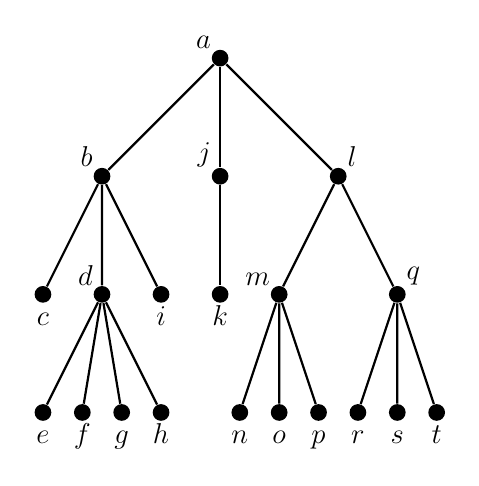
\begin{tikzpicture}[thick,scale=0.5, every node/.style={scale=0.5}, level distance=3cm]
    \tikzstyle{marrs}=[very thick,-latex]
    \tikzstyle{tnode}=[circle, fill=black, inner sep=1.5mm]
    \def\rstep{5cm}
    
    \huge
    
    \tikzstyle{level 1}=[sibling distance=3cm]
    \tikzstyle{level 2}=[sibling distance=1.5cm]
    \tikzstyle{level 3}=[sibling distance=1cm]
    
    \node[tnode] (a) {}
        child { node[tnode] (b) {} 
            child { node[tnode] (c) {} }
            child { node[tnode] (d) {} 
                child { node[tnode] (e) {} }
                child { node[tnode] (f) {} }
                child { node[tnode] (g) {} }
                child { node[tnode] (h) {} }
            }
            child { node[tnode] (i) {} }
        }
        child { 
            node[tnode] (j) {} 
            child { node[tnode] (k) {} }
        }
        child { node[tnode] (l) {} 
            child { node[tnode] (m) {} 
                child { node[tnode] (n) {} }
                child { node[tnode] (o) {} }
                child { node[tnode] (p) {} }
            }
            child[missing] {}
            child { node[tnode] (q) {} 
                child { node[tnode] (r) {} }
                child { node[tnode] (s) {} }
                child { node[tnode] (t) {} }
            }
        }
    ;
    \foreach \i in {c, e, f, g, h, i, k, n, o, p, r, s, t} {
        \node[below=8mm, anchor=base] at (\i) {$\i$};
    }
    \foreach \i in {a, b, d, j, m} {
        \node[above left] at (\i) {$\i$};
    }
    \foreach \i in {l, q} {
        \node[above right] at (\i) {$\i$};
    }
    
    
    
\end{tikzpicture}
  \caption{Дерево, представляющее список $a \ldots t$.}
  \label{fig:10.4}
\end{figure}

Функция \lstinline!head! проста:
\begin{lstlisting}
  fun head (C (x, _)) = x
\end{lstlisting}
Чтобы сконкатенировать два непустых списка, мы связываем два дерева,
делая второе из них последним ребёнком первого.
\begin{lstlisting}
  fun xs $\concat$ E = xs
    | E $\concat$ ys = ys
    | xs $\concat$ ys = link xs ys
\end{lstlisting}
Вспомогательная функция \lstinline!link! добавляет второй аргумент к
очереди детей первого аргумента.
\begin{lstlisting}
  fun link (C (x, q), ys) = C (x, Q.snoc (q, ys))
\end{lstlisting}
Функции \lstinline!cons! и \lstinline!snoc! просто вызывают $\concat$.
\begin{lstlisting}
  fun cons (x, xs) = C (x, Q.empty) $\concat$ xs
  fun snoc (xs, x) = xs $\concat$ C (x, Q.empty)
\end{lstlisting}
Наконец, имея непустое дерево, функция \lstinline!tail! должна
отбросить корень и каким-то образом превратить очередь детей в единое
дерево. Если очередь пуста, \lstinline!tail! должна вернуть
\lstinline!E!. В противном случае мы связываем всех детей вместе.
\begin{lstlisting}
  fun tail (C (x, q)) = if Q.isEmpty q then E else linkAll q
\end{lstlisting}
Поскольку конкатенация ассоциативна, мы имеем право связывать детей в
каком угодно порядке. Однако после небольшого размышления можно
заключить, что связывание детей справа налево, как показано на
Рис.~\ref{fig:10.5}, приведет к наименьшему повторению работы в
последующих вызовах \lstinline!tail!. Следовательно, мы реализуем
\lstinline!linkAll! как
\begin{lstlisting}
  fun linkAll q = let val t = Q.head q
                      val q' = Q.tail q
                  in if Q.isEmpty q' then t else link (t, linkAll q') end
\end{lstlisting}

\begin{remark}
  Функция \lstinline!linkAll! является примером программной схемы \lstinline!foldr1!.
\end{remark}

\begin{figure}
  \centering
  \begin{tikzpicture}[thick,scale=0.5, every node/.style={scale=0.5},level distance=2cm]
    
    \newcommand{\subtrg}[2]{\draw[thick] (#1.center) -- ++(0.6cm, -2cm) -- ++(-1.2cm, 0) -- cycle; \node[yshift=-1.8cm] at (#1.center) {#2}}

    
    \tikzstyle{tnode}=[circle, fill=black, inner sep=1.5mm]
    \tikzstyle{tnodes}=[circle, fill=black, inner sep=1.7mm, shift={(1.73cm, -1.73cm)}]
    \tikzstyle{level 1}=[sibling distance=2.3cm]
    
    \huge
    
    \begin{scope}
    
        \node[tnode] (x) {}
            child foreach \i in {a, b, c, d} { node[tnode] (\i) {} }
        ;
        \foreach \i in {a, b, c, d} {
            \subtrg{\i}{};
        }
        \node[above left] at (x) {$x$};
        \foreach \i in {a, b} {
            \node[left=2mm] at (\i) {$\i$};
        }
        \foreach \i in {c, d} {
            \node[right=2mm] at (\i) {$\i$};
        }
        \foreach \i in {0, 1, 2, 3} {
            \node[xshift=\i * 2.3cm, yshift=-2.5cm] at (a) {$t_\i$};
        }
    
    \end{scope}

    \node (rar) at (6cm, -2cm) {$\Longrightarrow$};
    \node[above=2mm] at (rar) {\texttt{tail}};
    \begin{scope}[shift={(8cm,2cm)}]
        \node[tnode] (a) {} 
            child { node[tnodes] (b) at (a) {}
                child { node[tnodes] (c) at (b) {}
                    child { node[tnodes] (d) at (c) {} }
                }
            }
        ;
        \foreach \i in {a, b, c, d} {
            \subtrg{\i}{};
            \node[above right] at (\i) {$\i$};
        }
        \foreach \i in {0, 1, 2, 3} {
            \node[xshift=\i * 1.73cm, yshift=-2.5cm - \i * 1.73cm] at (a) {$t_\i$};
        }
    \end{scope}
            
\end{tikzpicture}

  \caption{Операция \lstinline!tail!.}
  \label{fig:10.5}
\end{figure}
В этой реализации \lstinline!tail! может отнимать до $O(n)$
времени. Мы надеемся уменьшить этот показатель до амортизированного
$O(1)$, но чтобы добиться этого в условиях устойчивости,
нужно как-то ввести в нашу структуру ленивое вычисление. Поскольку
\lstinline!linkAll!~--- единственная процедура, требующая более, чем
$O(1)$ времени, она является естественным кандидатом. Мы переписываем
\lstinline!linkAll!, чтобы каждый рекурсивный вызов
задерживался. Задержка вынуждается, когда дерево извлекается из
очереди.
\begin{lstlisting}
  fun linkAll q = let val $\$$t = Q.head q
                      val q' = Q.tail q
                  in if Q.isEmpty q' then t else link (t, $\$$linkAll q') end
\end{lstlisting}
Чтобы это определение имело смысл, нужно, чтобы в очередях содержались
не просто деревья, а задержанные деревья, так что мы переопределяем
тип как
\begin{lstlisting}
  datatype $\alpha$ Cat = E | C of $\alpha$ $\times$ $\alpha$ Cat susp Q.Queue
\end{lstlisting}
Чтобы соответствовать этому новому типу, операция $\concat$ должна
задерживать свой второй аргумент.
\begin{lstlisting}
  fun xs $\concat$ E = xs
    | E $\concat$ xs = xs
    | xs $\concat$ ys = link (xs, $\$$ys)
\end{lstlisting}
Полная реализация приведена на Рис.~\ref{fig:10.6}.

\begin{figure}
  \centering
  
  \caption{Списки с конкатенацией.}
  \label{fig:10.6}
\end{figure}

Очевидно, что \lstinline!head! работает за время $O(1)$ в худшем
случае, а \lstinline!cons! и \lstinline!snoc! имеют те же временные
характеристики, что и $\concat$. Мы доказываем, что $\concat$ и
\lstinline!tail! работают за амортизированное время $O(1)$ методом
банкира. Нераздельная стоимость этих операций $O(1)$, так
что нам нужно только показать, что каждая из них высвобождает не более
$O(1)$ единиц долга.

Пусть $d_t(i)$ будет количество единиц долга, приписанных к $i$-му
узлу дерева $t$, а $D_t(i) = \sum_{j=0}^i d_t(j)$~--- общая сумма
долга на узлах $t$ вплоть до $i$ включительно. Пусть, наконец, $D_t$
будет общая сумма долга на всех узлах $t$ (т.~е., $D_t = D_t(|t| -
1)$. Мы будем соблюдать два инварианта долга.

Во-первых, будем требовать, чтобы число единиц долга на каждом узле
было ограничено сверху степенью этого узла (т.~е., $d_t(i) \le
\mathit{degree}_t(i)$). Поскольку сумма степеней всех узлов непустого дерева на
единицу меньше размера этого дерева, это означает, что общая сумма
долга, приписанная к дереву, ограничена его размером (т.~е., $D_t <
|t|$). Этот инвариант мы будем поддерживать, увеличивая долг на узле
дерева только одновременно с увеличением его степени.

Во-вторых, мы требуем, чтобы величина $D_t(i)$ была ограничена
некоторой линейной функцией от $i$. Конкретная выбранная нами функция
такова:
$$
D_t(i) \le i + \mathit{depth}_t(i) 
$$
где $\mathit{depth}_t(i)$ есть длина пути от корня дерева $t$ до узла
$i$. Этот инвариант называется \term{лево-линейный инвариант
  долга}{left-linear debit invariant}. Заметим, что лево-линейный
инвариант долга гарантирует нам, что $d_t(0) = D_t(0) \le 0 + 0 = 0$,
так что ко времени, когда узел оказывается корнем, весь долг на нём
уже выплачен. (На самом деле, корень даже не является задержкой!)
Единственное место, где мы вынуждаем задержки~---  когда задержанная
вершина становится новым корнем.

\begin{theorem}\label{th:10.1}
  Операции $\concat$ и \lstinline!tail! сохраняют оба инварианта
  долга, высвобождая, соответственно, одну и три единицы.

  \emph{Доказательство.} ($\concat$) Единственная единица долга,
  создаваемая функцией $\concat$~--- для тривиальной задержки её второго
  аргумента. Поскольку степень этого узла не увеличивается, мы
  немедленно высвобождаем эту единицу.  Предположим теперь, что $t_1$
  и $t_2$ непусты, и что $t = t_1 \concat t_2$. Пусть $n =
  |t_1|$. Заметим, что индекс, глубина и общее количество единиц долга
  на всех вершинах $t_1$ не затрагиваются конкатенацией, так что для
  $i < n$,
  $$
  \begin{array}{lcl}
    D_t(i) & = & D_{t_1}(i) \\
           & \le & i + \mathit{depth}_{t_1}(i) \\
           & = & i + \mathit{depth}_t(i) \\
  \end{array}
  $$
  Индекс каждой вершины в $t_2$ увеличивается на $n$, глубина
  увеличивается на единицу, а количество единиц долга увеличивается на
  общий долг $t_1$, так что
  $$
  \begin{array}{lcl}
    D_t(n+i) & = & D_{t_1} + D_{t_2}(i) \\
             & < & n + D_{t_2}(i) \\
             & \le & n + i + \mathit{depth}_{t_2}(i) \\
             & = & n + i + \mathit{depth}_t(n+i) - 1 \\
             & < & n + i + \mathit{depth}_t(n+i) \\
  \end{array}
  $$
  Таким образом, чтобы сохранить лево-линейный инвариант, больше
  никакие единицы долга высвобождать не требуется.

  (\lstinline!tail!) Пусть $t' = \lstinline!tail! t$. Отбросив корень
  $t$, мы связываем его детей $t_0 \ldots t_{m-1}$ справа
  налево. Пусть $t'_j$ будет частичный результат связывания $t_j
  \ldots t_{m-1}$. Тогда $t' = t'_0$.  Поскольку все операции
  связывания, кроме последней, задерживаются, мы присваиваем по одной
  единице долга корню каждого $t_j$, $0 < j < m-1$. Заметим, что
  степень каждого из этих узлов увеличивается на единицу.  Кроме того,
  одну единицу долга мы присваиваем корню $t'_{m-1}$ из-за того, что
  задерживается последний вызов \lstinline!linkAll!, хотя он и не
  вызывает \lstinline!link!.  Поскольку степень этого узла не
  меняется, мы немедленно высвобождаем эту последнюю единицу долга.

  Предположим теперь, что $i$-й узел дерева $t$ оказывается в дереве
  $t_j$. Исходя из лево-линейного инварианта долга, мы знаем, что
  $D_t(i) < i + \mathit{depth}_t(i)$, однако рассмотрим теперь, как
  каждая из величин изменяется при применении операции
  \lstinline!tail!. $i$ уменьшается на единицу, поскольку
  отбрасывается первый элемент. Глубина каждого узла в $t_j$
  увеличивается на $j-1$ (см. Рис.~\ref{fig:10.5}), а общее число
  единиц долга на каждом узле $t_j$ увеличивается на $j$. Таким
  образом,
  $$
  \begin{array}{lcl}
    D_{t'}(i-1) & = & D_t(i) + j \\
                & \le & i + \mathit{depth}_t(i) + j \\
                & = & i + (\mathit{depth}_{t'}(i-1) - (j-1)) + j \\
                & = & (i-1) + \mathit{depth}_{t'}(i-1) + 2 \\
  \end{array}
  $$
  Высвобождение первых двух единиц долга восстанавливает инвариант,
  так что всего получается высвобождено три единицы.
\end{theorem}

\begin{hint}
  Если имеется хорошая реализация очередей, то наши списки с
  конкатенацией~--- лучшая из известных устойчивых реализаций этой структуры, особенно
  для приложений, существенно опирающихся на устойчивость.
\end{hint}

\begin{exercise}\label{ex:10.6}
  Напишите функцию \lstinline!flatten! с типом 
  \lstinline!$\alpha$ Cat list $\to$ $\alpha$ Cat!, конкатенирующую
  все элементы списка списков с конкатенацией. Покажите, что Ваша
  функция работает за амортизированное время $O(1+e)$, где $e$~---
  число пустых списков с конкатенацией в исходном списке.
\end{exercise}

\subsection{Кучи с эффективным слиянием}
\label{sc:10.2.2}

В этом разделе мы используем структурную абстракцию для куч и получаем
эффективную операцию слияния.

Допустим, у нас есть реализация куч, поддерживающая \lstinline!insert!
за время $O(1)$ в худшем случае, а \lstinline!merge!,
\lstinline!findMin! и \lstinline!deleteMin! за время $O(\log n)$ в
худшем случае. Одна такая реализация~--- скошенные биномиальные кучи
из Раздела~\ref{sc:9.3.2}; ещё одна~--- биномиальные кучи с
расписанием из Раздела~\ref{sc:7.3}. При помощи структурной абстракции
мы собираемся улучшить время работы операций \lstinline!merge! и
\lstinline!findMin! до $O(1)$ в худшем случае.

Предположим пока что, что тип куч полиморфен относительно типа
элементов, и что для любого типа элементов мы магическим образом
знаем, какую функцию сравнения использовать. Позже мы учтём, что как
тип элементов, так и функция сравнения на этих элементах задаются в
момент применения функтора.

С учётом перечисленных предположений тип развёрнутых куч можно задать
как
\begin{lstlisting}
  datatype $\alpha$ Heap = E | H of $\alpha$ $\times$ ($\alpha$ Heap) PrimH.Heap
\end{lstlisting}
где \lstinline!PrimH!~--- реализация элементарных куч. Элемент,
хранимый в каждом узле \lstinline!H!, будет минимальным элементом
поддерева с корнем в этом узле. Элементами элементарных куч будут
служить развёрнутые кучи. Внутри элементарных куч развёрнутые кучи
упорядочены по своим минимальным элементам (т.~е., корням). Можно
думать об этом типе как о типе деревьев с переменной степенью
ветвления, причем дети каждого узла сами по себе хранятся в
элементарных кучах.

Поскольку минимальный элемент хранится в корне, функция
\lstinline!findMin! проста:
\begin{lstlisting}
  fun findMin (H (x, _)) = x
\end{lstlisting}
Чтобы слить две развёрнутые кучи, мы помещаем кучу с большим корнем в
кучу с меньшим корнем как элемент.
\begin{lstlisting}
  fun merge (E, h) = h
    | merge (h, E) = h
    | merge (h$_1$ as H (x, p$_1$), H$_2$ as H (y, p$_2$)) =
        if x < y then H (x, PrimH.insert (h$_2$, p$_1$))
        else H (y, H.insert (h$_1$, p$_2$))
\end{lstlisting}
(В выражении $x < y$ мы предполагаем, что функция $<$~--- правильная
функция сравнения для этих элементов.) \lstinline!insert!
определяется через \lstinline!merge!.
\begin{lstlisting}
  fun insert (x, h) = merge (H (x, PrimH.empty), h)
\end{lstlisting}
Наконец, рассмотрим \lstinline!deleteMin!, определённую как
\begin{lstlisting}
  fun deleteMin (H (x, p)) =
        if PrimH.isEmpty p then E
        else let val (H (y, p$_1$)) = PrimH.findMin p
                 val p$_2$ = PrimH.deleteMin p
             in H (y, PrimH.merge (p$_1$, p$_2$)) end
\end{lstlisting}
Отбросив корень, сначала мы смотрим, пуста ли элементарная куча
\lstinline!p!. Если да, то новая куча также пуста. В противном случае
мы находим и извлекаем минимальный элемент \lstinline!p!, являющийся
развернутой кучей с минимальным из всех элементом; этот элемент
становится новым корнем. Наконец, мы сливаем \lstinline!p$_1$! и
\lstinline!p$_2$! и получаем новую элементарную кучу.

Анализ этих куч не представляет сложности. Очевидно, что
\lstinline!findMin! работает за время $O(1)$ в худшем случае
независимо от нижележащей реализации элементарных куч. Функции
\lstinline!insert! и \lstinline!merge! зависят только от
\lstinline!PrimH.insert!.  Поскольку мы предполагаем, что время работы
\lstinline!PrimH.insert! равно $O(1)$ в худшем случае, таково же и
время работы \lstinline!insert! и \lstinline!merge!. Наконец, 
\lstinline!deleteMin! вызывает \lstinline!PrimH.findMin!,
\lstinline!PrimH.deleteMin! и \lstinline!PrimH.merge!. Поскольку все
они работают за $O(\log n)$ в худшем случае, такова же и
характеристика \lstinline!deleteMin!.

\begin{remark}
  Можно также разворачивать кучи с амортизированными ограничениями
  производительности. Например, развёртка ленивых биномиальных куч из
  Раздела~\ref{sc:6.4.1} даёт нам реализацию, поддерживающую
  \lstinline!findMin! за время $O(1)$ в худшем случае, операции
  \lstinline!insert! и \lstinline!merge! за амортизированное время
  $O(1)$, а \lstinline!deleteMin! за амортизированное время $O(\log n)$.
\end{remark}

До сиз пор мы предполагали, что тип куч полиморфен, но на самом деле
сигнатура \lstinline!Heap! указывает, что кучи мономорфны~--- как тип
элементов, так и функция сравнения этих элементов фиксируются в момент
применения функтора. Реализация кучи~--- это функтор,
параметризованный типом элементов и функцией сравнения. Функтор,
который мы используем для развёртки куч, отображает функторы куч в
функторы куч, а не структуры куч в структуры куч. Мы можем выразить
это с помощью функторов высших порядков \cite{MacQueenTofte1994}:
\begin{lstlisting}
  functor Bootstrap (functor MakeH (Element : Ordered)
                              : Heap where type Elem.T = Element.T)
                    (Element : Ordered): Heap = $\ldots$
\end{lstlisting}
Функтор \lstinline!Bootstrap! принимает функтор \lstinline!MakeH! в
качестве параметра. Функтор \lstinline!MakeH! принимает структуру
\lstinline!Element! с сигнатурой \lstinline!Ordered!, определяющей тип
элементов и функцию сравнения, и возвращает структуру
\lstinline!Heap!. При заданном \lstinline!MakeH!,
\lstinline!Bootstrap! возвращает функтор, который принимает структуру
\lstinline!Element! с сигнатурой \lstinline!Ordered! и возвращает
структуру \lstinline!Heap!.

\begin{remark}
  Ограничение \lstinline!where type! в сигнатуре функтора
  \lstinline!MakeH! необходимо, чтобы гарантировать, что функтор
  возвращает структуру кучи с необходимым типом элементов. Ограничения
  такого рода чрезвычайно часто встречаются в функторах высших порядков.
\end{remark}

Теперь, чтобы создать структуру элементарных куч с развёрнутыми кучами
в качестве элементов, мы применяем функтор \lstinline!MakeH! к
структуре \lstinline!BootstrappedElem! с сигнатурой
\lstinline!Ordered!, определяющей тип развёрнутых куч и функцию
сравнения, упорядочивающую две развёрнутые кучи по их минимальным
элементам. (Отношение порядка не определено на двух пустых кучах.) Это
можно выразить при помощи следующих двух взаимно рекурсивных
объявлений.
\begin{lstlisting}
  structure rec BootstrappedElem =
    struct
      datatype T = E | H of Elem.T $\times$ PrimH.Heap
      fun leq (H (x, _), H (Y, _)) = Elem.leq (x, y)
      $\mbox{\ldots Подобные же определения для }$ eq $\mbox{и}$ lt $\ldots$
    end
  and PrimH = MakeH (BootstrappedElem)
\end{lstlisting}
где \lstinline!Elem!~--- структура с сигнатурой \lstinline!Ordered!,
определяющая подлинные элементы развёрнутой кучи.  Полная реализация
функтора \lstinline!Bootstrapped! приведена на Рис.~\ref{fig:10.7}.

\begin{figure}
  \centering
  (* $\mbox{Рекурсивные структуры не поддерживаются в Стандартном ML!}$ *)\\
  $\mbox{\ldots Подобные же определения для }$ eq $\mbox{и}$ lt $\ldots$\\
  (* $\mbox{Экспортируются конструкторы }$ E $\mbox{и}$ H *)\\
  \caption{Развёрнутые кучи.}
  \label{fig:10.7}
\end{figure}

\begin{remark}
  В Стандартном ML запрещены рекурсивные определения структур, и этот
  запрет оправдан: это объявление не имеет смысла для функторов
  \lstinline!MakeH!, имеющих эффекты. Однако функторы
  \lstinline!MakeH!, к которым мы можем пожелать применить
  \lstinline!Bootstrap!, например, \lstinline!SkewBinomialHeap! из
  Раздела~\ref{sc:9.3.2}, в этом отношении вполне безопасны, и
  рекурсивный шаблон, воплощаемый функтором \lstinline!Bootstrap!, для
  них имеет смысл. Жаль, что Стандартный ML не дает нам выразить
  развёртку таким образом.

  Развёрнутые кучи всё же можно реализовать в Стандартном ML, если
  явно подставить конкретную реализацию \lstinline!MakeH!, скажем,
  \lstinline!SkewBinomialHeap! или \lstinline!LazyBinomialHeap!, а
  затем избавиться от отдельных структур \lstinline!BootstrappedElem!
  и \lstinline!PrimH!. Тогда рекурсия на структурах сводится к
  рекурсии на типах данных, которая Стандартным ML  поддерживается.
\end{remark}

\begin{exercise}\label{ex:10.7}
  Подстановка функтора \lstinline!LazyBinomialHeap! из
  Раздела~\ref{sc:6.4.1}, как указано выше, приводит к типам
  \begin{lstlisting}
    datatype Tree = Node of int $\times$ Heap $\times$ Tree list
    datatype Heap = E | NE of Elem.T $\times$ Tree list susp
  \end{lstlisting}
  Завершите эту реализацию развёрнутых куч.
\end{exercise}

\begin{exercise}\label{ex:10.8}
  Часто в элементах кучи содержится информация помимо приоритета. Для
  таких типов элементов часто бывает удобно использовать кучи,
  хранящие приоритет отдельно от остального содержимого элемента. На
  Рис.~\ref{fig:10.8} приведена альтернативная сигнатура для такого
  типа куч.
  \begin{enumerate}
  \item Приспособьте либо \lstinline!LazyBinomialHeap!, либо
    \lstinline!SkewBinomialHeap! к этой сигнатуре.
  \item Перепишите функтор \lstinline!Bootstrap! как
    \begin{lstlisting}
      functor Bootstrap (PrimH : HeapWithInfo) : HeapWithInfo = $\ldots$
    \end{lstlisting}
    Вам не потребуются ни функторы высших порядков, ни рекурсивные
    структуры.
  \end{enumerate}
\end{exercise}

\begin{figure}
  \centering
  
  \caption{Альтернативная сигнатура для куч.}
  \label{fig:10.8}
\end{figure}

\section{Развёртка до составных типов}
\label{sc:10.3}

Мы видели несколько примеров, где коллекции составных данных
(например, кучи куч) оказывались полезными для реализации коллекций
простых данных (например, кучи элементов). Однако коллекции составных
данных часто бывают полезны сами по себе.  Простой пример: строки
(т.~е., последовательности символов) часто служат типом
элементов множеств или ключами в конечных отображениях. В этом разделе
мы иллюстрируем развёртку конечных отображений, определённых для
какого-то простого типа, до конечных отображений, определённых на
списках или даже на деревьях, составленных из элементов этого типа.

\subsection{Префиксные деревья}
\label{sc:10.3.1}

Двоичные деревья поиска хорошо работают, когда операция сравнения для
типа ключа или элемента дёшева. Это условие выполняется для простых
типов вроде целых чисел и символов, но для составных типов вроде строк оно
может оказаться неверным. Рассмотрим, например, представление
телефонной книги с помощью двоичного дерева поиска. Обработка запроса
<<Кузнецов, Владислав>> может потребовать множество сравнений с
записями <<Кузнецов, Владимир>>, и каждое из этих сравнений будет
проверять десяток символов в каждой строке, прежде чем вернуть
результат.

Для составных типов лучшим решением будет выбрать представление,
которое использует структуру конкретного типа. Одним из таких
представлений является \term{префиксное дерево}{trie}, известное также
как \term{цифровое дерево поиска}{digital search tree}. В этой главе
мы с помощью префиксного дерева реализуем абстракцию
\lstinline!FiniteMap! (конечное отображение), показанную на Рис.~\ref{fig:10.9}.

\begin{figure}
  \centering
  
  (* $\mbox{Если ключ не найден, возбудить }$ NotFound *)
  \caption{Сигнатура для конечных отображений.}
  \label{fig:10.9}
\end{figure}

В последующем обсуждении мы будем предполагать, что ключи являются
строками, и что представлены они как списки символов. Мы часто будем
называть символы \term{базовым типом}{base type}. Основные идеи легко
распространить на другие типы последовательностей и другие базовые
типы. 

Префиксное дерево~--- это дерево с переменной степенью ветвления, и
каждая дуга в нем помечена символом. Дуги, исходящие из корня дерева,
представляют первый символ строки; дуги, исходящие из прямых потомков
корня, представляют второй символ, и так далее. Чтобы найти узел,
соответствующий данной строке, нужно начать с корня и двигаться по
дугам, помеченным символами строки по порядку.  Например, префиксное
дерево, представляющее строки \lstinline!"cat"!, \lstinline!"dog"!,
\lstinline!"car"! и \lstinline!"cart"!, можно изобразить как
\begin{center}
  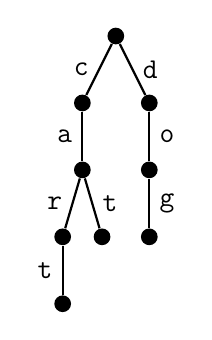
\begin{tikzpicture}[thick,scale=0.5, every node/.style={scale=0.5}, level distance=1.7cm]
    \tikzstyle{marrs}=[very thick,-latex]
    \tikzstyle{tnode}=[circle, fill=black, inner sep=1.5mm]
    \def\rstep{5cm}
    
    \huge
    \tt
    
    \tikzstyle{level 1}=[sibling distance=1.7cm]
    \tikzstyle{level 3}=[sibling distance=1cm]
    
    \node[tnode] {}
        child { node[tnode] {} 
            child { node[tnode] {}
                child { node[tnode] {} 
                    child { node[tnode] {} 
                        edge from parent node[left] {t}
                    }
                    edge from parent node[left] {r}
                }
                child { node[tnode] {} 
                    edge from parent node[right] {t}
                }
                edge from parent node[left] {a}
            }
            edge from parent node[left] {c}
        }
        child { node[tnode] {}
            child { node[tnode] {}
                child { node[tnode] {} 
                    edge from parent node[right] {g}
                }
                edge from parent node[right] {o}
            }
            edge from parent node[right] {d}
        }
        
        ;
    
    
    
    
\end{tikzpicture}
\end{center}
Заметим, что при вставке строки в префиксное дерево в него также
попадают все префиксы этой строки. Только некоторые из этих префиксов
будут соответствовать реальным записям.  В нашем примере префиксами
строки \lstinline!"cart"! являются \lstinline!"c"!, \lstinline!"ca"! и \lstinline!"car"!, но
из них реальная запись соответствует только строке \lstinline!"car"!. Поэтому
каждый узел требуется помечать как пустой или полный. В случае
конечных отображений мы для этого используем встроенный тип данных
\lstinline!option!.
\begin{lstlisting}
  datatype $\alpha$ option = None | Some of $\alpha$
\end{lstlisting}
Если узел пуст, мы помечаем его значением \lstinline!None!. Если же
узел полон, и соответствующая строка отображается в значение
\lstinline!x!, мы помечаем узел значением \lstinline!Some x!.

Остаётся важный вопрос, как нам представлять дуги, исходящие из
вершины. Обычно мы бы представляли непосредственных потомков вершины с
переменной степенью ветвления в виде списка, однако здесь нам также
требуется хранить метки дуг. В зависимости от выбора базового типа и
ожидаемой плотности префиксного дерева, дуги, исходящие из узла, можно
представлять в виде вектора, ассоциативного списка, двоичного дерева
поиска или даже, если базовый тип сам по себе является списком или
строкой, в виде ещё одного префиксного дерева! Однако все эти типы
представляют из себя всего лишь конечные отображения из меток дуг в
префиксные деревья. Мы абстрагируемся от конкретного представления
отображений на дугах, предполагая, что нам дана некоторая
структура \lstinline!M!, реализующая конечные отображения для базового
типа. В таком случае, представлением для префиксного дерева
оказывается
\begin{lstlisting}
  datatype $\alpha$ Map = Trie of $\alpha$ option $\times$ $\alpha$ Map M.Map
\end{lstlisting}
Пустое дерево представлено как одиночная пустая вершина без потомков.
\begin{lstlisting}
  val empty = Trie (None, M.empty)
\end{lstlisting}
Чтобы найти строку, мы ищем каждый её символ в соответствующем
отображении дуг. Дойдя до последнего узла, мы проверяем, пуст он или
полон.
\begin{lstlisting}
  fun lookup ([], Trie (None, m)) = raise NotFound
    | lookup ([], Trie (Some x, m)) = x
    | lookup (k :: ks, Trie (v, m)) = lookup (ks, M.lookup (k, m))
\end{lstlisting}
Заметим, что когда строка отсутствует в префиксном дереве, мы не
всегда даже дойдём до последнего узла. Например, если в
вышеприведённом примере мы будем искать слово \lstinline!"dark"!, мы
найдём букву \texttt{d}, но не найдём \texttt{a}. При этом функция
\lstinline!M.lookup! возбудит исключение
\lstinline!NotFound!. Поскольку это исключение также является
правильным ответом на \lstinline!lookup!, мы его просто распространяем
дальше.

\begin{remark}
  Из-за такого поведения при неудачном поиске префиксные деревья могут
  оказаться даже быстрее, чем хэш-таблицы. Неудачный поиск по
  префиксному дереву может завершиться, просмотрев только несколько
  первых символов, в то время как неудачный поиск по хэш-таблице
  требует просмотра всей строки только для того, чтобы вычислить хэш-функцию!
\end{remark}

Функция записи в дерево \lstinline!bind! очень похожа на
\lstinline!lookup!, только здесь мы не позволяем \lstinline!M.lookup!
окончиться неудачно. Мы подставляем пустой узел каждый раз, когда она
возбуждает исключение \lstinline!NotFound!.
\begin{lstlisting}
  fun bind ([], x, Trie (_, m)) = Trie (Some x, m)
    | bind (k :: ks, x, Trie (v, m)) = 
        let val t = M.lookup (k, m) handle NotFound $\Rightarrow$ empty
            val t' = bind (ks, x, t)
        in Trie (v, M.bind (k, t', m)) end
\end{lstlisting}
Полная реализация приведена на Рис.~\ref{fig:10.10}.

\begin{figure}
  \centering
  
  \caption{Простая реализация префиксных деревьев.}
  \label{fig:10.10}
\end{figure}

\begin{exercise}\label{ex:10.9}
  Очень часто множество ключей, которые нужно хранить в префиксном
  дереве, обладает свойством, что ни один ключ не может быть префиксом
  другого. Например, все ключи могут иметь одну и ту же длину, либо
  все ключи могут заканчиваться на один и тот же символ, который ни в
  одной другой позиции не встречается. Реализуйте префиксные деревья
  заново, предполагая, что это условие выполняется, и используя тип
  \begin{lstlisting}
    datatype $\alpha$ Map = Entry of $\alpha$ | Trie of $\alpha$ Map M.Map
  \end{lstlisting}
\end{exercise}

\begin{exercise}\label{ex:10.10}
  В префиксных деревьях часто встречаются длинные цепочки узлов,
  каждый из которых имеет только по одному потомку. Существует
  оптимизация, когда все эти узлы сливаются в один. Этого можно
  добиться, храня в каждом узле подстроку-наибольший общий префикс
  всех ключей, путь к которым пролегает через этот узел. В таком
  случае, тип префиксных деревьев будет
  \begin{lstlisting}
    datatype $\alpha$ Map = Trie of M.key list $\times$ $\alpha$ option $\times$ $\alpha$ Map M.Map
  \end{lstlisting}
  Реализуйте префиксные деревья, используя этот тип. Следует соблюдать
  инвариант, что узел не может одновременно быть пустым и являться
  единственным потомком. Можно предполагать, что структура
  \lstinline!M! содержит функцию \lstinline!isEmpty!.
\end{exercise}

\begin{exercise}\label{ex:10.11}
  \textbf{(Швенке \cite{Schwenke1997})} Есть ещё одна структура,
  использующая многослойные конечные отображения~---
  \term{хэш-таблица}{hash table}. Завершите следующую реализацию
  абстрактных хэш-таблиц.
  \begin{lstlisting}
    functor HashTable (structure Approx : FiniteMap,
                       structure Exact  : FiniteMap,
                       val hash : Exact.Key $\to$ Approx.Key) : FiniteMap =
    struct
       type Key = Exact.Key
       type $\alpha$ Map = $\alpha$ Exact.Map Approx.Map
       $\ldots$
       fun lookup (k, m) = Exact.lookup (k, Approx.lookup (hash k, m))
       $\ldots$
    end
  \end{lstlisting}
  Преимущество этого представления состоит в том, что в
  \lstinline!Approx! мы можем использовать эффективный тип ключа
  (скажем, целые числа), а в \lstinline!Exact! можно использовать
  тривиальное представление (например, ассоциативные списки).
\end{exercise}

\subsection{Обобщенные префиксные деревья}
\label{sc:10.3.2}

Идею префиксных деревьев можно обобщить со списков на другие составные типы,
например, деревья \cite{ConnellyMorris1995}. Рассмотрим
сначала, как отображения дуг в предыдущем разделе отражают тип
конструктора \lstinline!cons!. Отображения дуг представлены типом
\lstinline!$\alpha$ Map M.Map!. Внешнее отображение индексирует первое
поле конструктора \lstinline!cons!, а внутреннее отображение~--- второе
поле конструктора \lstinline!cons!. Поиск головы
\lstinline!cons!-ячейки во внешнем отображении даёт нам внутреннее
отображение, и в нём мы ищем хвост ячейки \lstinline!cons!.

Мы можем обобщить эту схему на двоичные деревья, имеющие три поля,
добавив третий слой отображений. Например, если у нас есть двоичные деревья
типа
\begin{lstlisting}
  datatype $\alpha$ Tree = E | T of $\alpha$ $\times$ $\alpha$ Tree $\times$ $\alpha$ Tree
\end{lstlisting}
то мы можем представлять отображения дуг в префиксных деревьях по этим
деревьям как \lstinline!$\alpha$ Map Map M.Map!. Внешнее отображение
индексирует первое поле конструктора \lstinline!T!, среднее
отображение~--- второе поле, а внутреннее отображение индексирует
третье поле. Поиск элемента в каком-либо узле во внешнем отображении
даёт нам среднее отображение, где мы можем искать левое
поддерево. Этот поиск, в свою очередь, даст нам внутреннее
отображение, и там мы можем искать правое поддерево.

Более формально, мы представляем префиксные деревья над бинарными
деревьями типом
\begin{lstlisting}
  datatype $\alpha$ Map = Trie of $\alpha$ option $\times$ $\alpha$ Map Map M.Map
\end{lstlisting}
Заметим, что здесь мы имеем гетерогенный рекурсивный тип, так что в
функциях, работающих с этим типом, нам потребуется полиморфная
рекурсия.

Функция \lstinline!lookup! проводит три поиска на каждый конструктор
\lstinline!T!, соответствующих трём полям конструктора. Когда она
достигает последнего узла, проводится проверка, полон ли этот узел.
\begin{lstlisting}
  fun lookup (E, Trie (None, m)) = raise NotFound
    | lookup (E, Trie (Some x, m)) = x
    | lookup (T (k, a, b), Trie (v, m)) = 
        lookup (b, lookup (a, M.lookup (k, m)))
\end{lstlisting}
Функция \lstinline!bind! работает подобным же образом. Она показана на
Рис.~\ref{fig:10.11}, где приведена полная реализация префиксных
деревьев поверх двоичных деревьев.

\begin{figure}
  \centering
  (* $\mbox{предполагает полиморфную рекурсию!}$ *)  
  \caption{Обобщённые префиксные деревья.}
  \label{fig:10.11}
\end{figure}

\begin{exercise}\label{ex:10.12}
  Реализуйте функтор \lstinline!TrieOverTrees! без использования
  полиморфной рекурсии, на основе типов
  \begin{lstlisting}
    datatype $\alpha$ Map = Trie of $\alpha$ EM option $\times$ $\alpha$ Map M.Map
    datatype $\alpha$ EM = Elem of $\alpha$ | Map of $\alpha$ Map
  \end{lstlisting}
\end{exercise}

\begin{exercise}
  Реализуйте префиксные деревья, ключами в которых служат деревья с
  переменной степенью типа
  \begin{lstlisting}
    datatype $\alpha$ Tree = T of $\alpha$ $\times$ $\alpha$ Tree list
  \end{lstlisting}
\end{exercise}

Имея эти примеры, мы можем обобщить понятие префиксного дерева до
любого рекурсивного типа, включающего произведения и суммы. Требуется
только несколько простых правил о том, как сконструировать конечное
отображение для структурного типа, имея в качестве основы конечные
отображения для его компонент. Пусть \lstinline!$\alpha$ Map$_\tau$!
будет тип конечных отображений над типом $\tau$.

В случае произведений мы уже знаем, что делать; чтобы найти пару в
префиксном дереве, нужно сначала найти первый элемент этой пары и
получить отображение, где следует искать второй элемент. Таким
образом,
$$
\tau = \tau_1 \times \tau_2 \Rightarrow 
\lstinline!$\alpha$ Map$_\tau$! =
  \lstinline!$\alpha$ Map$_{\tau_2}$ Map$_{\tau_1}$!
$$
Что же делать с суммами? Вспомним тип деревьев и префиксных деревьев
над ними:
\begin{lstlisting}
  datatype $\alpha$ Tree = E | T of $\alpha$ $\times$ $\alpha$ Tree $\times$ $\alpha$ Tree
  datatype $\alpha$ Map = Trie of $\alpha$ option $\times$ $\alpha$ Map Map M.Map
\end{lstlisting}
Ясно, что тип \lstinline!$\alpha$ Map Map M.Map! соответствует
конструктору \lstinline!T!, но что соответствует конструктору
\lstinline!E!? Тип \lstinline!$\alpha$ option! представляет собой не
что иное, как очень эффективную реализацию конечных отображений над
типом \lstinline!unit!, который, в свою очередь, эквивалентен
отсутствующему телу конструктора \lstinline!E!. Отсюда мы выводим
общее правило для сумм:
$$
\tau = \tau_1 + \tau_2 \Rightarrow 
\lstinline!$\alpha$ Map$_\tau$! =
\lstinline!$\alpha$ Map$_{\tau_1}$ $\times$ $\alpha$ Map$_{\tau_2}$!
$$

\begin{exercise}\label{ex:10.14}
  Завершите следующие функторы, которые реализуют вышеописанные
  правила для произведений и сумм:
  \begin{lstlisting}
    functor ProductMap (M$_1$ : FiniteMap) (M$_2$ : FiniteMap) : FiniteMap =
    struct
          type Key = M$_1$.Key $\times$ M$_2$.Key
          $\ldots$
    end

    datatype ($\alpha$, $\beta$) Sum = Left of $\alpha$ | Right of $\beta$
    functor SumMap (M$_1$ : FiniteMap) (M$_2$ : FiniteMap) : FiniteMap =
    struct
          type Key = (M$_1$.Key, M$_2$ Key) Sum
          $\ldots$
    end
  \end{lstlisting}
\end{exercise}

\begin{exercise}\label{ex:10.15}
  Пусть имеется структура \lstinline!M!, реализующая конечные
  отображения над типом идентификаторов \lstinline!Id!. Реализуйте
  префиксные деревья над типом лямбда-выражений \lstinline!Exp!, где
  \begin{lstlisting}
    datatype Exp = Var of Id | Lam of Id $\times$ Exp | App of Exp $\times$ Exp
  \end{lstlisting}
  В процессе решения полезно будет расширить тип префиксных деревьев отдельным
  конструктором для пустого отображения.
\end{exercise}

\section{Примечания}
\label{sc:10.4}

\noindent
\textbf{Развёртка структур данных} Развёртка структур данных была
распознана как общая методика проектирования структур данных в
работах Бухсбаума и его коллег \cite{Buchsbaum1993,
  BuchsbaumTarjan1995, BuchsbaumSundarTarjan1995}. Структурная
декомпозиция и структурная абстракция использовались и раньше,
соответственно в \cite{Dietz1982} и \cite{DriscollSleatorTarjan1994}.

\noindent
\textbf{Списки с конкатенацией} Несмотря на то, что построить
альтернативное представление устойчивых списков, поддерживающих
эффективную операцию конкатенации, относительно легко (см., например,
\cite{Hughes1986}), такие альтернативные представления, казалось,
почти неизбежно приносили в жертву эффективность функций
\lstinline!head! или \lstinline!tail!.

Майерс \cite{Myers1982} описывает представление, основанное на
AVL-деревьях, поддерживающее все основные операции за время $O(\log
n)$. Тарджан с коллегами \cite{DriscollSleatorTarjan1994,
  BuchsbaumTarjan1995, KaplanTarjan1995} исследовали множество
сублогарифмических представлений. Кульминацией из работы стало
представление, поддерживающее конкатенацию и все остальные обычные
функции над списками за время $O(1)$ в худшем случае. Реализация
списков с конкатенацией из Раздела~\ref{sc:10.2.1} впервые появилась в
\cite{Okasaki1995a}. Она намного проще, чем у Каплана и Тарджана, но
дает лишь амортизированные ограничения, а не жёсткие.

\noindent
\textbf{Кучи со слиянием} Многие императивные реализации поддерживают
операции \lstinline!insert!, \lstinline!merge! и \lstinline!findMin!
за амортизированное время $O(1)$, а операцию \lstinline!deleteMin! за
амортизированное время $O(\log n)$, включая биномиальные кучи
\cite{KhoongLeong1993}, фибоначчиевы кучи \cite{FredmanTarjan1987},
расслабленные кучи \cite{Driscoll-etal1988}, V-кучи
\cite{Peterson1987}, скошенные снизу вверх кучи
\cite{SleatorTarjan1986b} и парные кучи
\cite{Fredman-etal1986}. Однако из всех этих структур, кажется, только
парные кучи сохраняют свою амортизированную эффективность в сочетании
с ленивым порядком вычисления и устойчивостью
(см. Раздел~\ref{sc:6.5}), и, к сожалению, даже для парных куч
скоростные характеристики являются только недоказанным предположением.

Бродал \cite{Brodal1995, Brodal1996} достигает аналогичных ограничений
в худшем случае. Его исходная структура данных \cite{Brodal1995} может
быть реализована чисто функциональным образом (и, таким образом,
сделана устойчивой), если сочетать её с методикой рекурсивного
замедления Каплана и Тарджана \cite{KaplanTarjan1995}, а также с чисто
функциональной реализацией деков реального времени, вроде приведенной
в Разделе~\ref{sc:8.4.3}. Однако такая реализация будет
очень сложной и медленной. Бродал и Окасаки упрощают эту реализацию в
\cite{BrodalOkasaki1996}, используя скошенные биномиальные кучи
(Раздел~\ref{sc:9.3.2}) и структурную абстракцию (Раздел~\ref{sc:10.2.2}).

\noindent
\textbf{Полиморфная рекурсия} Существует несколько попыток расширить
Стандартный ML полиморфной рекурсией, например, \cite{Myers1984,
  Henglein1993, KfouryTiurynUrzyczyn1993}. Одна из сложностей
состоит в том, что при наличии полиморфной рекурсии вывод типов
становится формально неразрешимым \cite{Henglein1993, KfouryTiurynUrzyczyn1993},
хотя на практике он и работает. Язык Haskell обходит эту проблему,
позволяя полиморфную рекурсию в случае, если программист явно
указывает сигнатуру типа.

%%% Local Variables: 
%%% mode: latex
%%% TeX-master: "pfds"
%%% End: 
